\documentclass[a4paper,11pt]{report}
\usepackage[french]{babel}
\usepackage[T1]{fontenc}
\usepackage[utf8]{inputenc}
\usepackage{lmodern}
\usepackage{microtype}
\usepackage{hyperref}
\usepackage{tabulary}
\usepackage{framed}
\usepackage{fancyhdr}
\usepackage{amsmath}
\usepackage{bbm}
\usepackage{graphicx}
\usepackage{pst-all}
\usepackage{xcolor}

%\usepackage{nopageno}

\newcommand{\latin}[1]{\textit{#1}}

\pagestyle{empty}

\pagestyle{fancy}
\fancyhead{}
\renewcommand{\headrulewidth}{0.5pt}
\fancyhead[R]{\textit{\nouppercase{\rightmark}}}
\fancyfoot{}
\renewcommand{\footrulewidth}{0.5pt}
\fancyfoot[L]{\textit{\nouppercase{\leftmark}}}
\fancyfoot[R]{\thepage}
  
\begin{document}
	\begin{titlepage}
		\vspace*{\stretch{2}}
		\begin{center}
			\large\bfseries\itshape Projet SAR\\
		\end{center}
		\noindent\rule{\linewidth}{3pt}

		\begin{center}
			\Huge\bfseries\itshape RAPPORT\\
		\end{center}
		
		\noindent\rule{\linewidth}{3pt}
		\begin{center}
			\bfseries
			\large Recherche de filtres de Bloom similaires \\
			\large Application à la recherche par mots clés basée sur une DHT
		\end{center}
		\vspace*{\stretch{2}}
		\begin{center}
			Réalisé par \textbf{NDOMBI TSHISUNGU} Christian \& \textbf{DOAN} Cao Sang \\
			Encadrant: M. \textbf{MAKPANGOU} Mesaac, Regal
		\end{center}
		\vspace*{\stretch{0.5}}
		\begin{center}
			26 Mars 2015
		\end{center}
	\end{titlepage}

\tableofcontents


\chapter{Introduction}
	{\Huge D}ans ce sujet, on abordera sur les recherches par mots clés. Une fois, on tape un mot ou une chaine de mots, l'application cherche dans la base de données pour trouver la liste des documents qui contient les descriptions correspondantes avec ces mots clés.
	
	Dans la base de données qui contient des grosses masses de donées, les index sont basés sur les descriptions des documents. Chaque mot est une clé, chaque clé contient une liste des documents ayant ce mot. Au contraire à la liste normale, le mot clé est le nom du document et il contient la liste des mots qui se trouvent dans la description de ce document. Par exemple, le mot {\em PSAR : le projet pour les étudiants du M1}, normalement, le mot clé est {\em PSAR}, donc il contient sa description {\em le projet pour les étudiants du M1}, mais dans cette liste, les mots clés sont {\em le, projet, pour, les, étudiants, du, M1} et chaque mot contient le mot {\em PSAR}. On s'appelle la {\em liste inversée}.
	
	Du coup, on utilise les tables de hachage distribuées (DHT) pour stocker les listes inversées. L'avantage d'utilisation de ces tables est que la complexité est égale à $ \theta ${\em (1)} car on trouve directement l'élément que l'on recherche. La statégie de distribution des listes inversées la plus utilisée (appelée partionnement vertical) consiste à associer à chaque terme une clé qui désigne le pair qu stocke la liste inversée associée à ce terme. Une fois que l'on lance la recherche sur les documents qui sont satisfaits à l'ensemble des mots que l'on a saisi, le système doit chercher pour chaque mot dans cet ensemble la liste des documents qui le contiennent, et puis fait l'intersection des listes inversées retrouvées. 

\chapter{Projet}
\section{Marché}
		Il existe actuellement plusieurs moteurs de recherche par mots clés sur le marché. Il est toujours nécessaire d’améliorer les recherches en minimisant le temps de réponse et le coût de recherche, d’autant plus que les besoins de recherche deviennent très importants lorsqu’on exploite des bases de données de plus en plus grande et complexe. L’application que nous développerons doit répondre explicitement à ces exigences.
		
	\section{Contexte et objectifs}
		Comme l’application FreeCore\cite{freecore}, qui utilise le filtre de Bloom pour faciliter la recherche par mot clé, le but de notre projet est d'explorer d’autres solutions basées sur une recherche de filtre de Bloom similaires.  Chaque filtre  de  Bloom  sera vu  comme  un  point  dans  un  espace à n dimensions  plutôt  qu'une  concaténation de  n mots binaires. On détermine ensuite une relation de proximité et on exploite les algorithmes de recherche des filtres similaires pour réduire l'ensemble de filtres à examiner.
		
	\section{Enoncé du besoin}
		Comme FreeCore, l’application exploitera les propriétés des filtres de Bloom. Il  permettra d’une part, de stocker les publications dans un fichier $VA\_file$ (put). Et d’autre part, d’effectuer des recherches de contenus par mots clés (search).
	\subsection{Stockage et indexation des publications}
	L’application permet de rechercher des publications qui contiennent tous les mots clés de la requête de façon optimale en utilisant le filtre de Bloom. Elle doit :
	\begin{itemize}
	
	\item créer un filtre de Bloom correspondant à la description de la publication, 
	\item créer un vecteur de n dimensions.
	\item créer les lieux où on stocke les différents documents,
	\item à partir d'un fichier de test, classer et indexer les documents dans les lieux correspondants,		
	\item ajouter un nouveau document à partir d'un filtre de Bloom,				\end{itemize}
	
	\subsection{Recherche de contenus}
	Pour la recherche l’application créera un Filtre de Bloom des mots clés, représentants notre critère de recherche, c’est-à-dire les mots clés et devra :
	\begin{itemize}
		\item recherche un document à partir du filtre de Bloom,
 		\item utilise le vecteur approximatif pour indexer et rechercher.
	\end{itemize}
	
En outre, l’application doit assurer les services suivants :

	\begin{itemize}
	\item afficher les messages d'erreurs, s'il en existe,	
	\item afficher les états de l'application,	
	\item interagir avec l'utilisateur,
	\item faciliter les tests en utilisant les fichiers de test ou en utilisant les entrées saisit par l'utilisateur.
	\end{itemize}
	\begin{description}
		\item[Note :] Nous ne traiterons pas les erreurs  possibles obtenues en cas de faute de frappe ou de faute d’orthographe, ni la différence de genre et de nombre des mots clés. Qui pourront faire objet d’une suite de ce travail.
			\end{description}

\chapter{Filtre de Bloom}
	{\huge \itshape U}n filtre de Bloom est une structure de données probabiliste compacte inventée par Burton Howard Bloom en 1970\footnote{Wikipédia}. L'avantage d'utilisation de filtre de Bloom est que cette technique nous permet de savoir avec certitude que l'élément n'est pas présenté dans l'ensemble d'élément, c'est-à-dire il ne faut pas y avoir de faux négatif mais il peut y avoir des faux positifs. On ne peut savoir qu'avec une certaine probabilité, l'élément peut être présent dans l'ensemble. Ce qui réduit d'une manière considérable les entrées lorsqu'on fait une recherche dans une masse de données. En plus, la taille de filtre est fixe et indépendante du nombre d'éléments contenus, par contre, plus déléments plus de faux positifs.
	
	En réalité, le filtre de Bloom a un structure très simple, un tableau B de \textit{m} bits associé à $i$ fonctions de hachage $h_i$, $0 \leq i \leq m - 1$ permettant de mapper tout élément de l'ensemble à une des $m$ cases du tableau. Ces fonctions de hachage ont une répartition uniforme des éléments de l'ensemble sur le tableau, et évidemment, doivent avoir une répartition différente. Au départ, le filtre représente un ensemble vide, et toutes les cases sont à 0.
	
	Pour chaque clé $k$ à ajouter à B, au lieu de se contenter de mettre à vrai la case B. $h(k)$ avec une seule fonction de hachage comme on le fait classiquement, on va mettre à vrai les $m$ cases B. $h_i(k)$. Le principe étant que la probabilité que deux clés différentes aient les mêmes $m$ valeurs pour leurs fonctions de hachage est faible.
	
	Pour savoir si une clé est présente, on s'assura que les $m$ cases de la table B correspondant aux valeurs des $m$ fonctions de hachage sont posisitionnées à $1$. Ce filtre est utile pour déterminer si un élément ne fait pas partie d'un ensemble, afin par exemple pour définir rapidement d'un traitement lourd lors de vérifier qu'une personne ne fasse pas partie d'une liste noire: d'abord, une vérification rapide avec le filtre de Bloom, puis en cas de potentiel posistif, un vérification plus certaine avec la comparaison dans la base de données.
	
	Le filtre de Bloom a quelques désavantages comme par exemple pour supprimer un élément dans l'ensemble de données, il nous faut reconstruire le filtre, en plus les faux posisitifs augmentent avec le nombre d'éléments présents dans l'ensemble. Nombreuses solutions utilisent des techniques probabilistes pour réduire le traitement d'information et leur coût.
	
	Le filtre de Bloom et leurs variantes sont largement utilisés dans divers systèmes distribués. Plusiseurs recherches récentes et beaucoup de nouveaux algorithmes ont été proposés pour les systèmes distribués qui sont directement ou indirectement basés sur Bloom filtres\cite{theory-and-practice-of-bloom-filters-for-distributed-systems}.
	
\newtheorem{algorithme}{Algorithme}
\begin{algorithme}
	Insertion dans le filtre de Bloom
\end{algorithme}

\begin{flushleft}
	\begin{framed}
		\textbf{IN:} \textit{x} objet à insérer dans le filtre de Bloom \textit{B}\\
		\textbf{FUNCTION:} \textit{insert(x)}\\
		\textbf{OUT:} $\emptyset$
		\noindent\rule{\linewidth}{0.5pt}

		\begin{tabbing}
			\textbf{for} \= $i = 0 ... k - 1$ \textbf{do}\\
					\> $j \leftarrow h_i(x)$\\
					\> \textbf{if} \= $B_j == 0$ \textbf{then}\\
					\> \> $B_j \leftarrow 1$\\
					\> \textbf{end}\\
			\textbf{end}
	    	\end{tabbing}		
	\end{framed}
\end{flushleft}
	
	Par exemple, supposons que nous souhaitions ajouter la clé "computer" dans la table B de taille 16 bits, que nous ayons 4 fonctions de hachage $ h_i, 0 \leq i < 4 $ et que $ h_0("computer") = 3$, $ h_1("computer") = 8$, $ h_2("computer") = 15$, $h_3("computer") = 10$, $h_4("computer") = 11 $. Donc, l'état de la table $ B $ après l'insertion sera:
	\begin{table}[!h]
		\centering		
		\begin{tabular}{|l|*{14}{c|}r|}
		\multicolumn{1}{c}{{\scriptsize 15}} &\multicolumn{1}{c}{}&\multicolumn{1}{c}{}&\multicolumn{1}{c}{}&\multicolumn{1}{c}{}&\multicolumn{1}{c}{}&\multicolumn{1}{c}{}&\multicolumn{1}{c}{}&\multicolumn{1}{c}{}&\multicolumn{1}{c}{}&\multicolumn{1}{c}{}&\multicolumn{1}{c}{}&\multicolumn{1}{c}{}&\multicolumn{1}{c}{}&\multicolumn{1}{c}{}&\multicolumn{1}{c}{{\scriptsize 0}}\\
		\hline
			1 & 0 & 0 & 0 & 1 & 1 & 0 & 1 & 0 & 0 & 0 & 0 & 1 & 0 & 0 & 0 \\
		\hline
		\end{tabular}
		\caption{Exemple filtre de Bloom}
		\label{filtredeBloom/exemple}
	\end{table}
	
\begin{algorithme}
	Test d'appartenance d'un élément dans le filtre
\end{algorithme}

\begin{flushleft}
	\begin{framed}
		\textbf{IN:} \emph{x} objet à tester dans le filtre de Bloom \textit{B}\\
		\textbf{FUNCTION:} \textit{ismember(x)}\\
		\textbf{OUT:} $bool$

		\noindent\rule{\linewidth}{0.5pt}

		\begin{tabbing}
			$m \leftarrow true$\\
			$i \leftarrow 0$\\
			\textbf{while} \= $m$ \&\& $i \leq k - 1$ \textbf{do}\\
					\> $j \leftarrow h_i(x)$\\
					\> \textbf{if} \= $B_j == 0$ \textbf{then}\\
					\> \> $m \leftarrow false$\\
					\> \textbf{end}\\
					\> $i \leftarrow i + 1$\\
			\textbf{end}
			\textbf{return} $m$\\
	    	\end{tabbing}		
	\end{framed}
\end{flushleft}

\begin{figure}[!htbp]
	\centering
	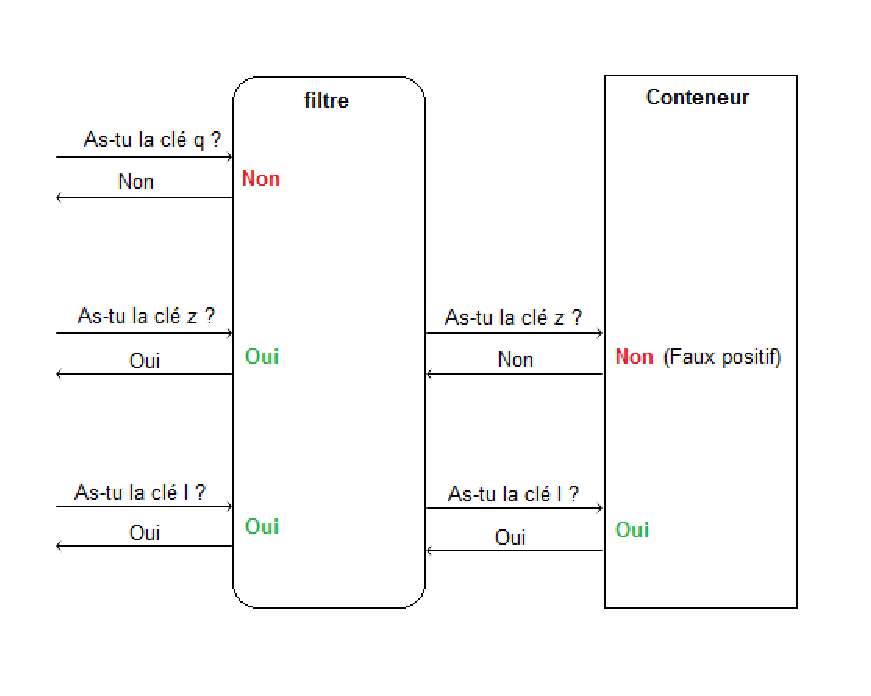
\includegraphics[width=12cm]{ismember.eps}
	\caption{isMember?}
\end{figure}	

	
	
	
	
	
	
	
	
	
	
	
	
	
	
	
	
	
	
	
	
	
\chapter{Réalisation du travail}
\section{Notre solution}
	{\huge \itshape N}ous avons choisi un filtre de Bloom de taille fixe de 512 bits, initialement rempli des 0 à chaque position. Pour générer un filtre de Bloom à partir de la description en entrée, le programme transforme chaque mot clé en 1 bit avec la position précise dans notre filtre. Nous avons utilisé une seule fonction de hachage basée sur SHA 256 bits, cette fonction encode un mot clé en une chaine hexadécimale de 256 bits. Avec un simple calcul, le filtre est bien rempli. Nous avons choisi seulement une fonction de hachage car si on en utilise plus d'une fonction, avec seulement un mot, on met sur plus d'une position le bit à 1, ce qui fait que, si on a par exemple 200 mots clés, comme c'est le cas des plusieurs entrées de notre fichier test, le filtre généré est rempli de 1. Ce problème rend imposible la réduction de l'ensemble des données de recherche. Et pourquoi doit-on ne pas augmenter la taille de filtre? Mais quelle taille suffit-il pour 200 descriptions si on a 3 fonctions de hachage? Après plusieurs tests et discussions ensemble, nous avons pris une seule fonction de hachage forte pour avoir moins de chance de collision. 
	
	En réalité, sur l'ensemble 107 459 documents, il existe au plus un document pour chaque filtre de Bloom, même s'il y a plusieurs documents qui ont plus de 200 mots dans leurs descriptions.
	
	Dans notre fichier test(benchmark), un document est une adresse URL décrite par l'ensemble de mots clés, ces mots clés sont écrits en codage UTF-8, en plusieurs langues et contiennent les caractères spéciales. Donc, pour chaque filtre de Bloom, nous avons créé le fichier qui contient seulement cette adresse URL. En utilisant encore une fois la fonction de hachage SHA 256 bits, elle nous rend le nom unique pour chaque document et les stocke sur le disque. Dans le cas le plus simple, pour ajouter un nouveau document, nous appliquons cette fonction de hachage pour chaque mot clé. 
	
	En appliquant encore une fois cette fonction sur le filtre de Bloom généré dans le premier temps, nous avons le fichier qui contient ce document qui correspond à ses mots clés. Ensuite, la recherche de document, facilement, on ré-applique cette fonction de hachage sur l'ensemble de mots clés pour trouver le filtre, à partir de ce filtre, on peut trouver le nom du fichier qui contient ce document. 
	
	Mais, cette solution marche si et seulement si on a exactement tous les mots clés dans la description d'un document, sinon cela ne marche jamais. Avec le filtre de Bloom, on peut savoir si ces mots clés existent dans l'ensemble des mots clés d'un document. Alors, pour chercher les documents qui contiennent ces mots clés, il faut regarder tous les filtres qui contiennent le filtre de la requête. Mais le parcours séquentiel est très lent sur le grand nombre de documents. 
	
\section{Indexation et stockage de données}
	{\huge \itshape P}our créer un index à partir d'un filtre, nous avons divisé chaque filtre de 512 bits en 64 morceaux de 8 bits. Pour chaque morceau, nous avons pris 4 bits de poids fort, donc, à la fin, nous avons un nouveau filtre de taille 256 bits, la taille de ce nouveau filtre est égale à la moitié de l'ancien filtre. On applique cette façon pour tous les filtres existants, si deux filtres de taille 512 bits qui génèrent le même filtre de taille 256 bits, ces deux filtres ont même index. Pour chaque index, on crée un fichier qui correspond avec cet index (\-nous utilisons la fonction SHA 256 aussi pour générer le nom de ce fichier), contient les filtres de taille 512 bits qui ont cet index. Après la création des index, on trouve le nombre des fichiers index sont beaucoup moins que celui des fichiers de document. On a $2^{256}$ valeurs possibles pour les index au lieu de $2^{512}$ valeurs différents avec le filtre de 512 bits. $2^{256}$ est un nombre très grand, mais heureusement un très grand nombre d'index non distribué.
	
	Pour éviter la recherche inutile sur les index inexistants, nous avons utilisé un tableau qui contient tous les index occupés. Ce tableau se situe dans le fichier $VA\_file$. La recherche devient plus facile et plus rapide car on calcule le filtre de taille 256 bits à partir de celui de taille 512 bits, ensuite, on cherche dans le fichier $VA\_file$ les index qui contient l'index de la requête, grâce à l'ensemble des index trouvés, on peut trouver les fichiers qui correspondent avec ces index pour trouver les filtres de taille 512 bits qui contiennent notre filtre de 512 bits. Si oui, on trouve l'ensemble des documents qui contient la requête. On note le filtre de Bloom de taille $k$ $B^k$, le filtre de la requête de taille $k$ $B^{k}_{req}$.
	
	Un \textit{VA\_file} peut finir par exploser s'il y a des milliers d'index. Le problème principal du coût et de temps de recherche se posera à nouveau. Pour résoudre ce problème, il faut limiter le nombre d'index à gérer dans le \textit{VA\_file}, en utilisant un nombre limite d'index pour chaque niveau d'index. Pour notre application, ce nombre est fixé à 1024 index par niveau d'indexation. Une fois, le nombre d'index stocké dans le $VA\_file$ dépasse ce seuil, l'application crée un nouveau niveau d'index. Ce nouveau d'index est référencé sur l'index plus bas. 
	
	Par exemple, un filtre de Bloom de taille 256 bits $B^{256}_1$ est l'index d'un filtre de Bloom de taille 512 bits $B^{512}_0$. Donc, pour chaque niveau $i$, le filtre créé doit satisfaire la formule suivant: $B^{\frac{512}{2^i}}_i$. 
	
	Le système recherche le fichier \textit{VA\_file} pour trouver les index existants. Chaque nouveau d'index \textit{i} correspond avec un fichier qui contient les index de niveau \textit{i - 1} qui ont le même nouveau d'index. Le système va refaire chaque fois que le seuil est dépassé.
	
	Est-ce que le niveau d'index est illimité? La réponse est non. Pour le filtre de Bloom que nous avons choisi 512 bits, nous avons maximum 6 niveaux, $B^{8}_6$. Du coup, la taille de filtre de Bloom au niveau le plus haut est de 8 bits. A ce niveau, on a au maximum 256 valeurs d'index possibles dans le fichier $VA\_file$, un nombre très petit par rapport au quantité de données. 
	
	La technique d'augmentation le niveau dynamique est très efficace si on a un nombre de données n'est pas important. Si on a plus de 100 000 documents à ajouter, la création des fichiers nécessaires nous prend plusieurs heures pour les créer. Donc, si on connaît le nombre de données, on peut fixer combien de niveaux d'index nécessaire. Selon notre résultat sur un disque dur SSD, nous avons fixé 6 niveaux d'index, la création nous coûte seulement 15 minuites. Avec la curiosité, nous avons essayé de réaliser sur un disque dur 80Go utilisé l'interface SATA II, il prend plus d'une heure pour faire le même travail. Du coup, nous avons laissé à côté la technique de création dynamique, et fixé 6 niveaux d'index utilisés.	
	
\section{Recherche de données}
	{\huge \itshape P}uisque l'on a fixé le nombre de niveau, on connaît la taille du filtre de Bloom contenu dans le fichier \textit{VA\_file}. Sinon on peut lire ce fichier pour trouver quel niveau où on est. D'abord, le système crée le filtre de Bloom de taille 512 bits $B^{512}_{req}$ pour la requête à partir de l'ensemble de mots clés fourni par l'utilisateur. A partir de ce filtre, le système calcul l'index de niveau le plus haut $B^{8}_{6_{req}}$ et lit le fichier $VA\_file$ pour trouver l'ensemble des index qui contiennent $B^{8}_{6_{req}}$. Une fois on a trouvé, le résultat est stocké dans un fichier $res_6$ qui correspond à ce niveau, ici c'est niveau 6. Ensuite, le système lit ce fichier de résultat pour trouver le nom des fichiers d'index à niveau 6 $B^{8}_{6}$, il accéde à ces fichiers et compare avec le filtre de la requête au niveau 5 $B^{16}_{5_{req}}$ avec les filtres trouvés. Car le fichier $VA\_file$ contient les index de niveau 6, chaque fichier qui correspond avec un index à niveau 6, contient les index de niveau 5, etc... Le résultat trouvé est stocké dans un fichier $res_5$. 
	
	Le système utilise la même façon en descendant vers le niveau 1. Le fichier $res_1$ contient les filtres de taille 256 bits $B^{256}_{1}$, en regardant les fichiers de $B^{256}_{1}$, on trouve les filtres de taille 512 bits $B^{512}_{0}$ et les compare avec le filtre $B^{512}_{req}$ de la requête, une fois que le filtre existant contient celui de la requête, on peut trouver facilement le nom du fichier qui contient le document cherché. Après la recherche, on trouve un ensemble de documents qui contient les mots clés de la requête. On ne peut éviter les faux positifs, on fait confiance à la puisance de fonction de hachage. Mais avec certitude, si un document ne contient pas la requête, il ne nous satisfait pas.

\chapter{Algorithme des fonctions}
\section{CREATE\_FILTER}
\begin{algorithme}
	Création d'un filtre de Bloom à partir d'un ensemble des descriptions
\end{algorithme}

\begin{flushleft}
	\begin{framed}
		\textbf{IN:} $\sum desc$\\
		\textbf{FUNCTION:} \textit{create\_filter($\sum desc$)}\\
		\textbf{OUT:} \textit{$B^{512}$}\\

		\noindent\rule{\linewidth}{0.5pt}

		\begin{tabbing}
			\textit{init($B^{512}$)}\\
			$x \leftarrow$ FIRST($\sum desc$)\\
			\textbf{while} \= $x \neq \emptyset$ \textbf{do}\\
					\> $i \leftarrow$ SHA\_256(\textit{x})\\
					\> $j \leftarrow i\ mod\ 512$\\
					\> $B^{512}[j]\leftarrow 1$\\
					\> $x \leftarrow$ NEXT($\sum desc$)\\
			\textbf{end}\\
			\textbf{return} $B^{512}$\\
	    	\end{tabbing}		
	\end{framed}
\end{flushleft}

\newpage
\section{PUT}
\begin{algorithme}
	Ajout d'un filtre dans le système
\end{algorithme}

\begin{flushleft}
	\begin{framed}
		\textbf{IN:} filtre de Bloom de taille 512 bits $B^{512}$\\
		\textbf{FUNCTION:} \textit{put($B^{512}$)}\\
		\textbf{OUT:} \textit{$\emptyset$}\\

		\noindent\rule{\linewidth}{0.5pt}

		\begin{tabbing}
			$i \leftarrow$ MAX\_LEVEL\\
			$vector_i \leftarrow$ CREATE\_VECTOR($B^{512}$, \textit{i})\\
			$x \leftarrow$ FIRST(\textit{VA\_file})\\
			\textbf{while }\= $x \neq \emptyset$ \textbf{do}\\
					\> \textbf{if }\= $vector_i = x$\textbf{ then}\\
					\> \> BREAK\\
					\> \textbf{end}\\
					\> $x \leftarrow$ NEXT(\textit{VA\_file})\\
			\textbf{end}	\\	
			
			\textbf{if }\= $vector_i \neq x$\textbf{ then}\\
				\> \textit{VA\_file } $\leftarrow$ ADD($vector_i$)\\
			\textbf{end}	\\	

			\textbf{for }\=$i = MAX\_LEVEL\ ...\ 1$ \textbf{do}\\
					\> \textbf{if }\= $i = 1$ \textbf{then}\\
					\> 	\> $vector_i \leftarrow$ CREATE\_VECTOR($B^{512}$, \textit{i})\\
					\>	\> CREATE\_FILE($vector_i,\ B^{512}$)\\
					\> \textbf{else}\\
					\>	\> $vector_i \leftarrow$ CREATE\_VECTOR($B^{512}$, \textit{i})\\
					\>	\> CREATE\_FILE($vector_i$, CREATE\_VECTOR($B^{512}$, \textit{i - 1}))\\
					\> \textbf{end}\\
			\textbf{end}	\\	
			\textbf{return} $\emptyset$\\
	    	\end{tabbing}		
	\end{framed}
\end{flushleft}

\newpage
\section{SEARCH}
\begin{algorithme}
	Recherche d'un document à partir d'un filtre de Bloom
\end{algorithme}

\begin{flushleft}
	\begin{framed}
		\textbf{IN:} filtre de Bloom de taille 512 bits $B^{512}_{req}$\\
		\textbf{FUNCTION:} \textit{search($B^{512}_{req}$)}\\
		\textbf{OUT:} \textit{$\sum doc$}\\

		\noindent\rule{\linewidth}{0.5pt}

		\begin{tabbing}
			$i \leftarrow$ MAX\_LEVEL\\
			$vector_i \leftarrow$ CREATE\_VECTOR($B^{512}_{req}$, \textit{i})\\
			$tmp \leftarrow$ CREATE\_FILE(\textit{i})\\
			$x \leftarrow$ FIRST(\textit{VA\_file})\\
			
			\textbf{while }\=$x \neq \emptyset $ \textbf{do}\\
					\> \textbf{if }\=$vector_i \subseteq x$ {then}\\
						\>\> tmp $\leftarrow$ ADD(\textit{x})\\
					\> \textbf{end}\\
					\> $x \leftarrow$ NEXT(\textit{VA\_file})\\
			\textbf{end}\\
			
			\textbf{for }\=$i = MAX\_LEVEL - 1\ ...\ 1$ \textbf{do}\\
					\> $vector_i \leftarrow$ CREATE\_VECTOR($B^{512}_{req}$, \textit{i})\\
					\> $x \leftarrow$ FIRST(FILE(\textit{i + 1}))\\
					\> $tmp \leftarrow$ CREATE\_FILE(\textit{i})\\
					\> \textbf{while }\=$x \neq \emptyset$\textbf{ do}\\
					\> \> $y \leftarrow$ FIRST(FILE(\textit{x}))\\
					\> \> \textbf{while }\= $y \neq \emptyset$ \textbf{ do}\\
					\> \> \> \textbf{if }\= $vector_i \subseteq y$\textbf{ then}\\
					\> \> \> \> tmp $\leftarrow$ ADD(\textit{y})\\
					\> \> \> \textbf{end}\\
					\> \> \> $y \leftarrow$ NEXT(FILE(\textit{x}))\\
					\> \> \textbf{end}\\
					\> \> $x \leftarrow$ NEXT(FILE(\textit{i + 1}))\\
					\> \textbf{end}\\
			\textbf{end}	\\
			$x \leftarrow$ FIRST(FILE(\textit{1}))\\
			\textbf{while }\=$x \neq \emptyset$\textbf{ do}\\
					\> $y \leftarrow $ FIRST(FILE(\textit{x}))\\
					\> \textbf{while }\= $y \neq \emptyset$\textbf{ do}\\
					\> \> \textbf{if }\= $B^{512}_{req} \subseteq y$\textbf{ then}\\
					\> \> \> $\sum doc \leftarrow$ ADD(FIRST(FILE(\textit{y})))\\
					\> \> \textbf{end}\\
					\> \> $y \leftarrow$ NEXT(FILE(\textit{x}))\\
					\> \textbf{end}\\
					\> $x \leftarrow$ NEXT(FILE(\textit{1}))\\
			\textbf{end}\\
			\textbf{return} $\sum doc$
	    	\end{tabbing}		
	\end{framed}
\end{flushleft}

\chapter{Résultat obtenu}
\section{Données}
	{\huge \itshape N}ous avons testé sur 107 459 documents, cette application a généré 319 720 fichiers nécessaires. 107 459 documents sont sous forme un lien URL. Au début, ces lien sont stockés dans un fichier de test. Nous avons testé le programme sur un processeur Intel Core\textsuperscript{\tiny{TM}} i7 2.3 GHz avec 8 Go de mémoire vive. Avant de chaque test, les fichiers temporaires se sont vidés.
	
\newpage
\section{Recherche aléatoire}
	{\huge \itshape P}our faire la recherche aléatoire, nous réalisons une requête avec les mots clés choisis aléatoirement. En augmentant le nombre de mots clés chaque fois que nous relançons la requête. Nous constatons que plus de mots clés, moins de temps d'attente de la réponse. Dans la figure \ref{recherche/aleatoire}, nous testons de un à 20 mots clés.

\begin{figure}[!htbp]
	\psset{linecolor=blue}
	\psset{xunit=0.5cm, yunit=0.1cm}
	\begin{pspicture}(-3,-1)(110,110)
		\psaxes[linewidth=1pt,linecolor=black,labels=none,ticks=none]{->}(0,0)(20.5,100)[$mot$,-90][$temps_{(s)}$,-180]
		\psline[linewidth=1.5pt](1,89.9)(2,54.9)(3,51.5)(4,40.4)(5,16.4)(6,5.8)(7,2.1)(8,1.3)(9,0.3)(10,0.3)(11,0.3)(12,0.3)(13,0.3)(14,0.3)(15,0.3)(16,0.3)(17,0.3)(18,0.3)(19,0.3)(20,0.3)
		\psline[linewidth=1pt,linecolor=black](1,1)(1,-1)\uput*[-90](1,0){1}
		\psline[linewidth=1pt,linecolor=black](2,1)(2,-1)\uput*[-90](2,0){2}
		\psline[linewidth=1pt,linecolor=black](8,1)(8,-1)\uput*[-90](8,0){8}
		\psline[linewidth=1pt,linecolor=black](0.15,89.9)(-0.15,89.9)\uput*[-180](0,89.9){89.9}
		\psline[linewidth=1pt,linecolor=black](0.15,54.9)(-0.15,54.9)\uput*[-180](0,54.9){54.9}
		\psline[linewidth=1pt,linecolor=black](0.15,1.3)(-0.15,1.3)\uput*[-180](0,1.3){1.3}
	\end{pspicture}
	\caption{Recherche aléatoire}
	\label{recherche/aleatoire}	
\end{figure}	

\newpage
\section{Recherche sélective}
	{\huge \itshape P}endant les tests, nous avons remarqué qu'avec le même nombre de mots clés inclut dans l'ensemble des mots clés de la description d'un document quelconque, le temps nécessaire pour avoir la réponse varie quand on change un mot clé par un autre du même ensemble. Le résultat est intéressant. Dans un premier temps, nous faisons le test avec un ensemble des mots clés qui appartiennent à plusieurs descriptions, nous les appellerons "populaire". Le deuxième test, nous ne prenons que les mots clés spécifiques à un document quelconque. La description d’un document dans ces deux tests reste identique, ce qui change est les mots clés utilisés. 

	Nous commençons par 1 mot et chaque fois nous relançons la requête, nous augmentons le nombre de mots clés. Dans le premier test, le nombre de mots clés augmenté ne signifie pas  le temps va être réduit. Dans le graphe, nous montrons que si on ajoute un mot "très populaire", ce mot nous coûte plus de temps. Dans le deuxième test, si on ajoute un mot "populaire" dans un ensemble des mots spécifique le temps augmente au lieu de diminuer. Ce mot casse l'advantage de la recherche sélective. 
	
	Donc, pour une meilleur recherche d'un document, il faut que nous cherchions plusieurs mots clés qui caractérisent le document d'une manière spécifique. Ce qui est difficile de gérer dans la réalité. La figure \ref{recherche/selective}, nous testons sur les requête d'un à sept mots clés. 
	
	\begin{figure}[!htbp]
		\psset{linecolor=blue}
		\psset{xunit=1cm, yunit=0.1cm}
		\begin{pspicture}(-3,-1)(110,110)
			\psaxes[linewidth=1pt,linecolor=black,labels=none,ticks=none]{->}(0,0)(8,100)[$mot$,-90][$temps_{(s)}$,-180]
			\psline[linecolor=red,linewidth=1.5pt](1,84.2)(2,89.1)(3,42.7)(4,64.4)(5,55.7)(6,62.2)(7,71.3)
			\psline[linecolor=blue,linewidth=1.5pt](1,84.2)(2,40.1)(3,37.4)(4,20.4)(5,17.7)(6,16.8)(7,0.8)
			\psline[linecolor=red,linewidth=1.5pt](3,100)(4,100) \uput*[0](4.3,100){\small{recherche avec les mots clés populaires}}
			\psline[linecolor=blue,linewidth=1.5pt](3,96)(4,96) \uput*[0](4.3,96){\small{recherche avec les mots clés caractéristiques}}
			\psline[linewidth=1pt,linecolor=black](1,1)(1,-1)\uput*[-90](1,0){1}
			\psline[linewidth=1pt,linecolor=black](0.08,84.2)(-0.08,84.2)\uput*[-180](0,84.2){\small{84.2}}
			\psline[linewidth=1pt,linecolor=black](2,1)(2,-1)\uput*[-90](2,0){2}
			\psline[linewidth=1pt,linecolor=black](0.08,89.1)(-0.08,89.1)\uput*[-180](0,89.1){\small{89.1}}
			\psline[linewidth=1pt,linecolor=black](0.08,40.1)(-0.08,40.1)\uput*{27pt}[-180](0,40.1){\small{40.1}}
			\psline[linewidth=1pt,linecolor=black](3,1)(3,-1)\uput*[-90](3,0){3}
			\psline[linewidth=1pt,linecolor=black](0.08,42.7)(-0.08,42.7)\uput*[-180](0,42.7){\small{42.7}}
			\psline[linewidth=1pt,linecolor=black](0.08,37.4)(-0.08,37.4)\uput*[-180](0,37.4){\small{37.4}}
			\psline[linewidth=1pt,linecolor=black](4,1)(4,-1)\uput*[-90](4,0){4}
			\psline[linewidth=1pt,linecolor=black](0.08,64.4)(-0.08,64.4)\uput*[-180](0,64.4){\small{64.4}}
			\psline[linewidth=1pt,linecolor=black](0.08,20.4)(-0.08,20.4)\uput*[-180](0,20.4){\small{20.4}}
			\psline[linewidth=1pt,linecolor=black](7,1)(7,-1)\uput*[-90](7,0){7}
			\psline[linewidth=1pt,linecolor=black](0.08,71.3)(-0.08,71.3)\uput*[-180](0,71.3){\small{71.3}}
			\psline[linewidth=1pt,linecolor=black](0.08,0.8)(-0.08,0.8)\uput*[-180](0,0.8){\small{0.8}}
		\end{pspicture}
		\caption{Recherche sélective}
		\label{recherche/selective}	
	\end{figure}

\chapter{Conclusion}
	{\huge \itshape A}près ce projet, notre technique de recherche a besoin d'ête amélioré, le temps de réponse est très important. Car la création d'un vecteur est une sorte de vecteur approximatif, mais ce vecteur ne définie pas forcément les caractéristiques du filtre donné. 
	
	Notre programme est écrit en C, donc la mémoire louée pour chaque programme est limité, nous ne pouvons stocker toutes les données intermédiaires dans la mémoire. Chaque fois nous obtenons un résultat intermédiaire, nous devons écrire sur le disque sous forme d'un fichier. Du coup, nous travaillons sur le disque dont le temps d'accès de disque nous coûte cher.
	
	En plus, notre travail est réalisé sur une seule machine, mais dans le réseau pair-à-pair, chaque machine se charge de gérer un niveau d'index par exemple, peut-être le temps de réponse sera plus court que sur une seule machine qui gère tous les niveaux.
	
	Ici, nous testons notre application un benchmark d'environ 100 000 documents seulement, si le nombre de données augmente, nous devons augmenter la taille de filtre et ajouter des nouvelles fonctions de hachage. Dans ces conditions notre technique de recherche répondra plus efficacement aux besoins de coût et de temps de réponse et assurera l'exactitude des documents trouvés.
	
	
	
	
	
	
	
	
	
	
	
\begin{thebibliography}{2}
	\bibitem{freecore}
		Mesaac Makpangou, Bassirou Ngom, Samba Ndiaye : 
		\textbf{\textit{Freecore: Un substrat d'indexation des filtres de Bloom fragmentés pour la recherche par mots clés}}.
		ComPAS'2014, Apr 2014, Neuchâtel, Switzerland
	\bibitem{theory-and-practice-of-bloom-filters-for-distributed-systems}
   		Sasu Tarkoma, Christian Esteve Rothenberg, and Eemil Lagerspetz :
  		 \textbf{\textit{Theory and Practice of Bloom Filters for Distributed Systems}}.
		Communications Surveys \& Tutorials, IEEE. pp. 131 – 155. Fevrier. 2012
\end{thebibliography}


\end{document}